\documentclass{IOS-Book-Article}

\usepackage{mathptmx}
\usepackage{graphicx}
\usepackage{subfigure}

%\usepackage{times}
%\normalfont
%\usepackage[T1]{fontenc}
%\usepackage[mtplusscr,mtbold]{mathtime}

\begin{document}
\begin{frontmatter}              % The preamble begins here.

%\pretitle{Pretitle}
\title{D\&C Matrix Assembly parallelization for Unstructured Meshes}
\runningtitle{D\&C Assembly}
%\subtitle{Subtitle}

\author[A]{\fnms{Lo\"ic} \snm{Th\'ebault}%
\thanks{Corresponding Author E-mail: }},
\author[A]{\fnms{Eric} \snm{Petit}},
\author[A]{\fnms{Marc} \snm{Tchiboukdjian}},
and
\author[B]{\fnms{Quang} \snm{Dinh}}

\runningauthor{L. Th\'ebault et al.}
\address[A]{PRISM - University of Versailles, France}
\address[B]{Dassault Aviation, Saint-Cloud, France}

\begin{abstract}
Current algorithms and runtimes struggle to scale to a large number of cores and show a poor parallel efficiency on current HPC machines.
The pure MPI codes are wasting IO, memory and communications. HPC users have to explore new paradigms to make an efficient usage of the new resources at their disposal such as hybrid MPI+threads.
In this paper we propose and evaluate a Divide \& Conquer, D\&C, approach for the parallelization on shared memory of an unstructured mesh assembly to sparse matrix.
Our target application is an industrial CFD application from Dassault Aviation computing mesh deformation for structure optimization.
The implementation is based on the versatile Cilk runtime and standard MPI. The original fortran code has been modified so that the elision of our modification is equivalent to the original pure MPI application.
Preliminary results on the matrix assembly of the application are encouraging and show good locality and scalability characteristics.
\end{abstract}

\begin{keyword}
Divide and Conquer, Task, Cilk, Mesh Partitioning, CFD, Matrix Assembly, FEM
\end{keyword}
\end{frontmatter}

\thispagestyle{empty}
\pagestyle{empty}

\section{Introduction}
%Positionment : code MPI compare to hybrid.\\
%Problem on FEM : assembling, parallelization with shared memory non trivial.\\
%Assembling on multicore, not on GPU (most of papers are for GPUs)\\\\

Current algorithms and runtimes struggle to scale on a large number of cores and show a poor parallel efficiency on current HPC machine. 
The major effects of the core count increase per node are a lower memory per core, higher requirement for concurrency (TLP, ILP, vector), higher coherency traffic and higher cost for coherency protocol.
The result is a severe challenge for performance scalability. The many-core accelerators such as the Xeon Phi exacerbate even more these issues.
HPC users have to explore new paradigms to make an efficient usage of the new resources at their disposal. 

In order to mitigate the node scalability issues, users can modify their application using hybrid MPI + thread to take advantage of the full topology of the machine and enhance the data and synchronization locality.
In this paper, we propose and evaluate a new parallelization strategy based on the Divide and Conquer, D\&C, principle. Our implementation is based on a task-based runtime, Cilk~\cite{cilk5}. 

We demonstrate the potential of the D\&C approach on the matrix assembly step from Finite Element Methods, FEM.
This step consists in building from the mesh the matrix describing the linear system to solve.
The values in the sparse matrix result from a reduction operation of some mesh elements.
The irregularity of the structure and the sequentialization of the reduction are challenging to achieve an efficient parallelization.
For multicores, except the state of the art coloring approaches, there is no recent research published on parallelizing matrix assembly.
In the manycore context, new algorithms are design for GPUs~\cite{Stanford,CPUGPUasm}, but can not be applied to shared multicores.

We apply our D\&C strategy for the parallelization of the matrix assembly on an industrial CFD code from Dassault Aviation computing the effect of mesh deformation to optimize the plane structure.
We compare our results to the original pure MPI implementation and the coloring approach for shared memory parallelization.
\\\\
The paper outline is the following:
\begin{itemize}
\item Section 2 presents the matrix assembly step in FEM applications using the coloring approach and our D\&C version using Cilk and MPI.
\item Section 3 presents the related works on recent FEM assembly methods and uses of D\&C principle on such FEM applications.
\item Section 4 presents the experimental setups and results on the assembly step of DEFMESH application from Dassault Aviation.
\item Section 5 is the conclusion and present our future works.
\end{itemize}

\section{Matrix Assembly}
%The process alterate the mesh geometry and be conservative of the mesh topology.  We have to work on a very unstructured mesh. Therefore, load balancing and interface
%computation prevent us to use geometrical domain decomposition.
%We use METIS~\cite{Metis} to do a topological domain decomposition that will not vary with the mesh deformation.
%The application iterates over three basic steps:
%\begin{itemize}
%\item Edge matrix assembly to CSR storage from the mesh coordinate array. This step potentially needs MPI communication in the case of using the elastic version.
%Explain in section ...
%\item Solve ... ??? what?
%\item Update the mesh coordinate and value, exchange the halo with other MPI rank.
%\end{itemize}

Matrix assembly is present in most of scientific applications using Finite Element Methods.
A simple assembly illustration on a 2D regular mesh is presented in figure~\ref{fig:2Dasm}.
To compute the value on $(N1,N2)$ edge, we have to sum the contributions of elements $E1$ and $E2$.
In 3D, the number of neighbor elements of an edge has no theoretical limits.

On an unstructured mesh, this step is non trivial to parallelize.
To create parallelism, one must create independent domains to work on.
In that case we envision two different approaches, a state-of-the-art coloring approach and our proposition of D\&C based on a topological recursive bisection.
\begin{figure}[htp]
 \centering
 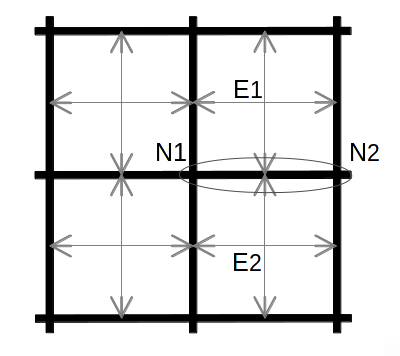
\includegraphics[scale=0.2]{2D_asm.png}
 \caption{2D assembling example}
 \label{fig:2Dasm}
\end{figure}

\subsection{Coloring}
\label{sec:col}
The coloring avoid race conditions by assigning a different color to elements sharing an edge.
Each element of a same color can be computed in parallel, but every color must be evaluated sequentially.
Although determining a minimal coloring is NP-complete, create a coloring with an undefined number of color is simple.
A pseudo-code is given in figure~\ref{fig:colApp} with a simple 2D coloring example.
\begin{figure}[htp]
 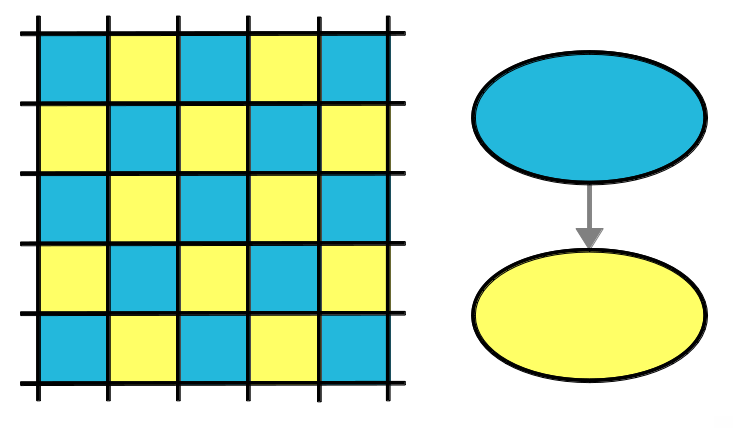
\includegraphics[scale=0.25]{Coloring_approach.png}
 \begin{verbatim}
 From initial Element_to_Node array, create:
 -> Node_to_Element array
 -> Element_to_Element array
 -> Element_to_Color array
 -> Color_to_Element array

 For each color - in sequential
     For all elements of current color - in parallel
         Compute element contribution
 \end{verbatim}
 \caption{Coloring approach}
 \label{fig:colApp}
\end{figure}
The main issue of coloring approach is the data locality. Indeed, elements of a same color are distant from each other and are not stored contiguously in memory.

\subsection{Divide \& Conquer}
%D\&C, approach on  unstructured meshes
%The rational is to divide recursively the work in two or more independent tasks, synchronize locally these tasks before returning. This recursive approach has many advantages.
%First the recursive sharing naturally exposes high concurrency. As long as the application is large enough, it is possible to produce a deeper tree to get more concurrency and 
%therefore match the higher requirement of many-core system. Furthermore synchronization are local: only nodes of a same parent node in the recursive
%tree needs to be synchronized. And finally, it greatly improved the data locality by reordering the data in smaller independent sets. 
%
%The D\&C approach is particularly interesting for its ability to scale naturally to an increasing number of node thanks to its architecture oblivious concept.
%Each leaves is responsible of its own data and there is a very minimal amount of sharing, avoiding costly locks and coherency protocols. 

The main idea of the D\&C approach for shared memory parallelization is to create task level parallelism while preserving a good data locality and minimizing synchronization cost.
Instead of increasing MPI domain decomposition and communications as data size increases, we increase the number of Cilk threads. MPI processes remain in moderate numbers.
In this way, we take benefit of the machine topology and most of communications are replaced by data sharing.
On a small number of cores, results of D\&C implementation are expected to be equivalent to pure MPI.
On a larger number of cores, the D\&C approach is expected to continue scaling, while pure MPI should loose in performance.

\subsubsection{Recursive Bisection}
D\&C is based on a topological recursive bisection of the mesh.
As illustrated in figure~\ref{fig:DCapp}, the left and right sub-domains created by these bisections are not sharing any element and thus, can be executed in parallel.
However, separator elements in the middle have nodes in both sides and must be treated after left and right sub-domains.
Therefore it is important to use a good partitioner to build equal sub-domains while minimizing the interface. In our case, we use the METIS graph partitioner~\cite{Metis}.
\begin{figure}[htp]
 \centering
 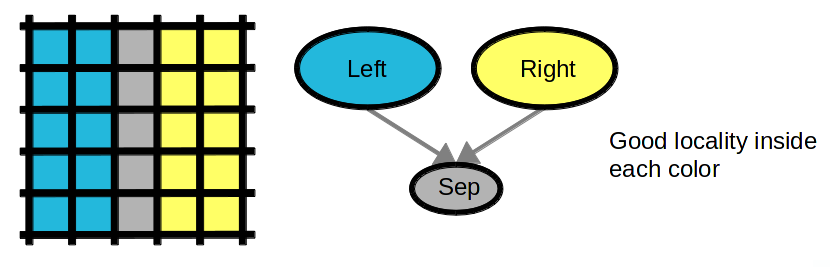
\includegraphics[scale=0.2]{DC_approach.png}
 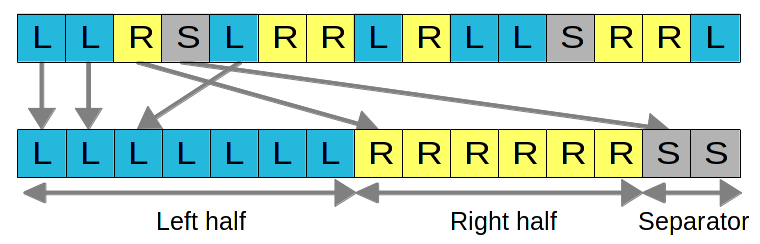
\includegraphics[scale=0.2]{Data_permutations.png}
 \caption{D\&C approach}
 \label{fig:DCapp}
\end{figure}

In order to increase the data locality, we also permute node and element arrays.
Indeed, nodes and elements can be consecutive in memory inside each sub-domain, improving intra-task locality.
Secondly, since the tasks distribution is following the recursive domain decomposition, we store neighbor sub-domains and associated separator contiguously to improve locality between tasks.

This approach is applied recursively to all sub-domains, offering a large amount of parallelism.
As illustrated in figure~\ref{fig:DCexe}, this results in a partition tree where each leaf is associated to an independent Cilk task.
\begin{figure}[htp]
 \centering
 \includegraphics[scale=0.2]{DC_rec.png}
 \includegraphics[scale=0.2]{DC_tree.png}
 \caption{D\&C recursive execution}
 \label{fig:DCexe}
\end{figure}

Otherwise, since the partitionment is topological, cuts are done on edges rather than geometrical coordinates.
This allows to compute sub-domains only once for a given mesh, despite of its deformations.
On next runs, the application needs only to apply the permutations before executing the recursive assembly.

\subsubsection{Cilk Implementation}
Cilk is a task based runtime developed by Intel. It allows to create parallel tasks with the \emph{spawn} keyword and to synchronize them with the \emph{sync} keyword.
All these tasks can be executed independently by threads. These threads, called \emph{workers}, have a queue of tasks to execute.
In order to improve the load balancing, Cilk runtime uses a work-stealing scheduler. Once a worker completes its queue, it can steal additional tasks from slower workers.

Starting from the tree shown in figure \ref{fig:DCexe}, the Cilk implementation is then straightforward.
Execution runs through the tree starting from the root and spawning a new Cilk task at each node separation.
This creates at each step of recursion parallelism between left and right parts.
Then, when recursion reaches a leaf, the code is simply running the sequential assembling on its sub-domain.
After left and right sub-domains are done, the corresponding Cilk tasks synchronize and one of them continue on the separator computation.
In order to have finer permutations without increase the number of Cilk tasks, it is also possible to stop the recursion earlier.
In this way, tasks no longer corresponds to leaves of the tree, but to nodes.
Thus, they execute sequentially and in one block the left, right and corresponding separator partitions which are stored contiguously in memory.

In some cases, when all elements or nodes are access in order inside a loop, there is no need to use a recursive task tree.
Indeed Cilk provides, as well as OpenMP, an easy way to parallelize loops using the \emph{cilk\_for} keyword.
By simply substituting the original \emph{for} by this keyword, iterations of the loop are split in several parallel tasks.
On the DEFMESH application, we observe a better scalability with the \emph{cilk\_for} than with \emph{OpenMP parallel for} pragma.

\subsubsection{To do}
explain problematic of sync, conherency, vecto (future work hybrid d\&c + coloring) etc.\\
explain compatibility with mpi\\

\section{Related Works}
Many choices are available to complete FEM assembly in parallel.
All methods have their advantages and their limitations, depending for instance on the target architecture or the mesh size.

Several studies \cite{Stanford,CPUGPUasm} investigates into different ways to compute FEM assembly on CPUs and GPUs.
One method consists in assembling by non-zero value of the system of equation. Several variants of this method exist.
A first one is to store contributions from mesh elements to global or local memory in parallel, and then reduce still in parallel these contributions to compute non-zero values.
By arranging data layout, this method can offer good performances. However, it can suffers of load imbalancing since requirement for non-zero values are heterogeneous.
Moreover, it can be very memory consuming and thus limited to small test cases.
An other variant consists to use one thread for the whole assembly step of one non-zero value at a time, but this approach leads to redundant computations.

An other method consists in assembling by mesh element \cite{CUDAfe,CPUfe1,CPUfe2}. One thread is responsible for the whole assembly step of one element at a time.
In order to launch several threads in parallel on independent elements, a coloring approach is often used.
In this way, each thread performs the same amount of computation, but suffers of poor performances because of a bad data locality as explained is section \ref{sec:col}.

An assembly approach for Recursive Sparse Blocks matrices have also been experimented \cite{RSBasm}, but seems to be highly memory-bandwidth bound.

\subsection{To do}
Atomics\\
Task Based parallelization SpMV, dongara and co \cite{MPI_task}\\

\section{Experiments}
To validate our approach, we apply the D\&C algorithm using Cilk and MPI on a the assembly step of an application from Dassault Aviation called DEFMESH.
We compare our results to the original pure MPI version of the assembly step and also to a MPI + OpenMP version which uses the coloring approach.

\subsection{Dassault Aviation DEFMESH Application}
The DEFMESH application is a Computational Fluid Dynamics (CFD) code based on a Finite Element Method (FEM).
It is used to apply deformations on an initial mesh in order to optimize its fluid flows.
It is fully parallelized with the MPI protocol and recently with OpenMP in few parts of the solver.
This solver is based on a conjugate gradient method and is mainly composed of dot products, SpMVs and reductions.

DEFMESH main kernel is decomposed in three steps.
First one is the assembly step where mesh data are gathered into a CSR structure.
Second step is the solver step which works on this CSR structure and computes optimal displacements.
Final step is the update of mesh coordinates using previously computed deformations.

Two versions of the kernel exist, a Laplacian version and an elastic version. Elastic version has a more complex assembly step and different boundary conditions for the solver (?).
While a simple scalar is computed for each edge of the mesh in the Laplacian version, a 3 by 3 matrix based on a more complex equation is computed in the elastic version.
Moreover, both versions can be whether linear or non linear.
The linear versions compute displacements in one step of deformation using the conjugate gradient methods as a direct method.
In the non linear versions, the deformation is split into a given number \emph{N} of smaller deformations.
The mesh is updated after each deformation and thus, each step of the kernel are repeated $N$times. The solver is then used as an iterative method.

We launch this application on two different test cases which are both irregular meshes from Dassault Aviation.
First one is a small mesh of 152 086 elements and 27 499 nodes which represents an M6 wing. We used it for developing and debugging.
Second test case, called EIB, is composed of 6 346 108 elements and 1 079 758 nodes. It represents the displacement of fuel tank along a plane fuselage.
This EIB test case has been used for experiments and measures presented in next section.

\subsubsection{To do}
nice picture of mesh deformation comparing variants\\
Communication for halo exchange\\

\subsection{Experimental Setups}
Experiments have been done on the Dassault Aviation EIB test case. It is an irregular mesh composed of 6 346 108 elements and 1 079 758 nodes.
It represents the displacement of fuel tank along a plane fuselage.

In the following experiments, we compare two versions of the DEFMESH application: the original one from Dassault Aviation called “Ref” and the new
Divide \& Conquer version called “D\&C”. The original version uses MPI between the different blocks of the mesh and OpenMP in some loops of the solver.
The D\&C version, as described above uses a recursive partitioning of each block of the mesh and exploits, in addition to MPI and OpenMP, a Cilk task parallelism
in the assembly step.

For each of these versions, we consider the two variants of DEFMESH: the Laplacian one and the elasticity one.
Both of them are non linear solvers with 50 steps of resolution. Measures correspond to the average time of one iteration.
In all cases we measure separately the assembly step, where the D\&C approach has been applied and the solving step, not yet modified.

We present the results both in terms of execution times and of parallel efficiency.
In all the graphics, the X axis represents the number of cores used. It corresponds to the product of MPI ranks by the number of Cilk / OpenMP threads.
In execution times graphics, the Y axis correspond either to RDTSC cycles (assembly step) or MPI\_Wtime seconds (solving step).
Concerning efficiency, the Y axis represents parallel efficiency given by the following formula:
$$Efficiency_{p-cores} = \frac{Time_{sequential}}{p*Time_{p-core}}$$
Graphics include the measures of the “Ref” and the “D\&C” versions.
For each of them, we use 1, 4, 8 and 12 MPI tasks and from 1 to 12 Cilk and OpenMP threads while the combination of MPI processes per Cilk/OMP threads is lower or equal to 12,
which correspond to the number of cores available. In all cases, the number of Cilk threads is equal to the number of OpenMP threads.
We also varied the number of METIS partitions and Cilk tasks in a large scope of values but we have not observed significant changes in the results.
Final values are 512 partitions and 128 Cilk tasks. This correspond to approximately 10 tasks per core, which is recommended in Cilk documentations.

All the experiments have been done with default the OpenMP affinity set to scatter and Cilk threads are not pinned. These experiments runs on an UVSQ server
composed of twelve cores distributed in two sockets of 6-cores Intel® Xeon® X5650 clocked at 2.67 GHz. The topology of the machine is described in the following illustration.
\begin{figure}[htp]
 \centering
 \label{fig5}
 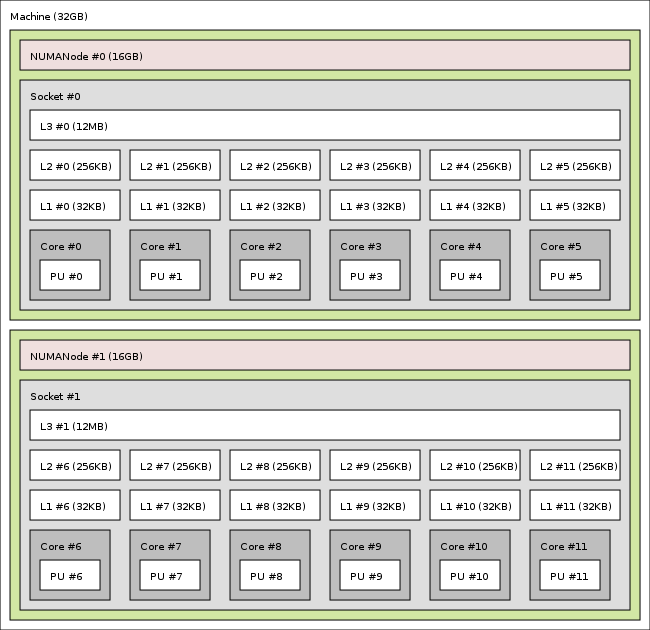
\includegraphics[scale=0.35]{topo_mauduit.png}
 \caption{UVSQ server topology}
\end{figure}

\subsection{Results}
\subsubsection{Laplacian Assembly}
\begin{figure}[htp]
 \centering
 \subfigure[Execution time]{\label{fig6:a}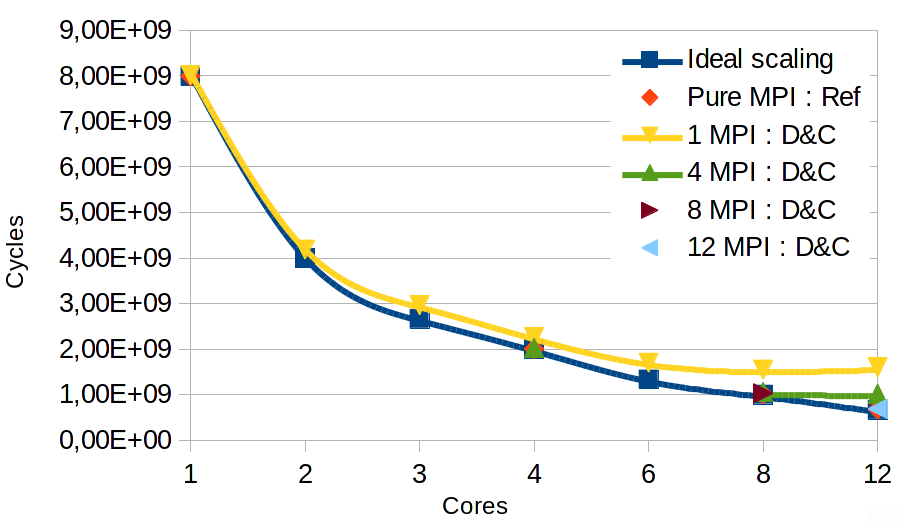
\includegraphics[scale=0.178]{Laplacian_asm_time.png}}\hspace{1em}%
 \subfigure[Parallel efficiency]{\label{fig6:b}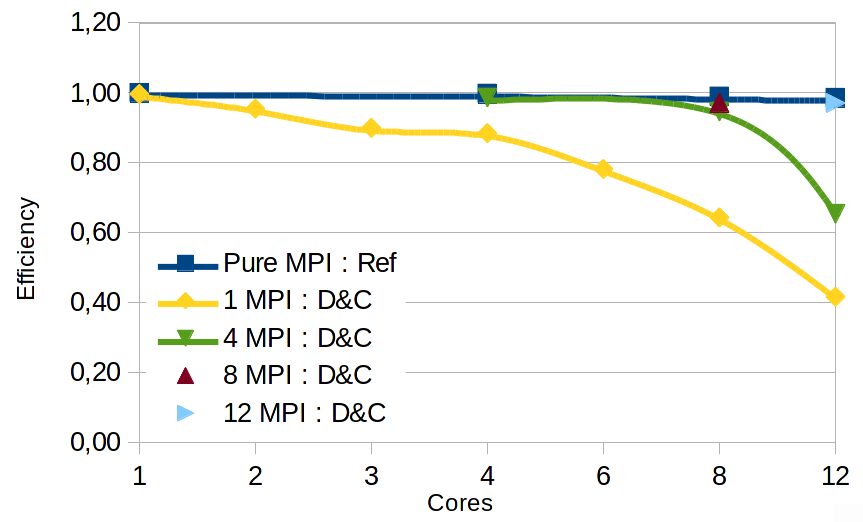
\includegraphics[scale=0.178]{Laplacian_asm_efficiency.png}}
 \caption{Laplacian assembly step}
\end{figure}
On the execution time curve, the D\&C approach is close to pure MPI but there is still a loss of efficiency beyond 6 cores.
This is probably due to the remaining sequential part of the D\&C code. Indeed, separator elements are not yet parallelized and can represent an important proportion
of the computation, especially for the one at the beginning of the recursion.

As we can see on the efficiency curve, the more the number of cores increase, the more the efficiency decrease. According to the Amdahl law,
the proportion of the sequential part over the parallel part is increasing with the number of cores. Moreover on the Laplacian solver, the amount of work for each
element in the assembly step is quite low and separators even less negligible. In the pure MPI version, this problem is not present since the whole mesh assembly is parallelized.

All in all, these first results are encouraging and we can reasonably expect to match the ideal scaling when the separators will be parallelized.

\subsubsection{Laplacian Solver}
\begin{figure}[htp]
 \centering
 \label{fig7}
 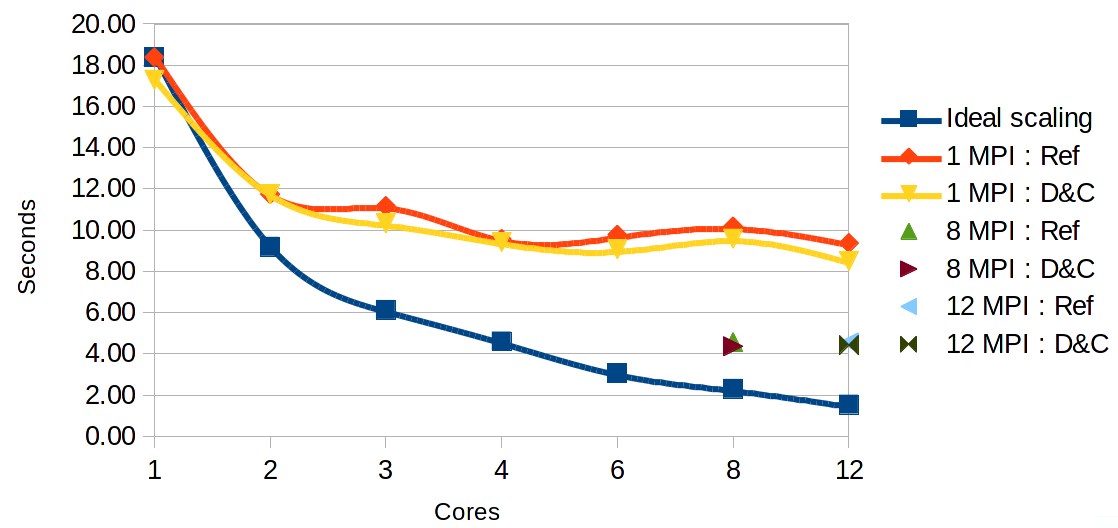
\includegraphics[scale=0.2]{Laplacian_solver_time.png}
 \caption{Laplacian solver execution time}
\end{figure}
The gains offered by the OpenMP parallelism are far from ideal scaling because of the small proportion of code parallelized in the solver.
Despite we did not modify the solver part, we observe a small benefit for the D\&C version compared to the reference version.
This gain is probably due to a better data locality generated by the permutations as explained in the previous section.
To confirm the locality hypothesis, we measured the L3 cache misses occurring during the solver and they are significantly lower with D\&C compared to the original version.
We also tried to permute data randomly and observe a degradation of performances.

\subsubsection{Elasticity Assembly}
\begin{figure}[htp]
 \centering
 \subfigure[Execution time]{\label{fig8:a}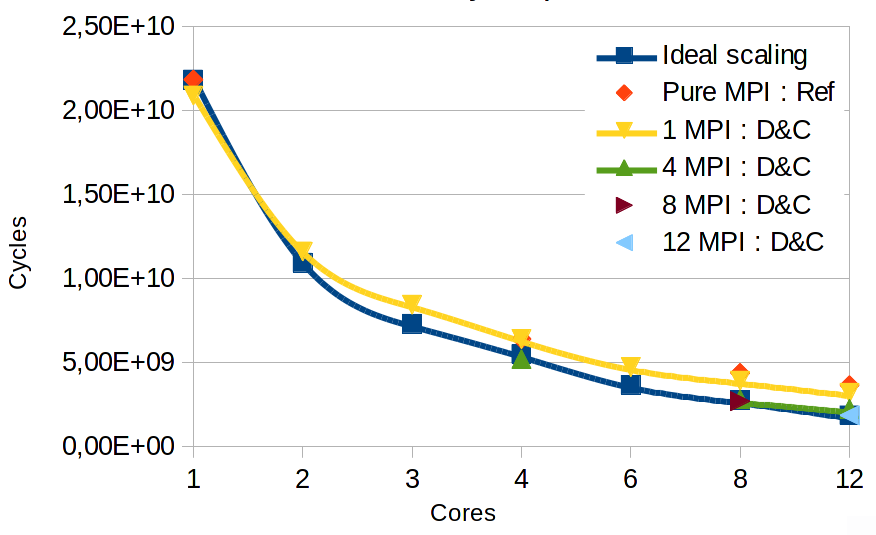
\includegraphics[scale=0.19]{Elasticity_asm_time.png}}\hspace{1em}%
 \subfigure[Parallel efficiency]{\label{fig8:b}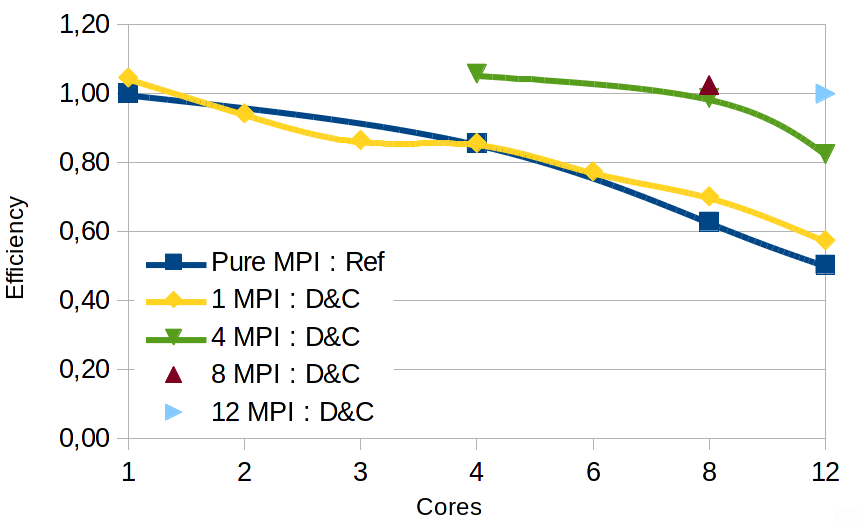
\includegraphics[scale=0.19]{Elasticity_asm_efficiency.png}}
 \caption{Elasticity assembly step}
\end{figure}
As we can see on the first curve, on the elasticity solver the D\&C approach is slightly faster than pure MPI and the parallel efficiency is equivalent.
In the elasticity case, the amount of work of the assembly step is bigger than the Laplacian.
Thus, the sequential part (ie separators computing) is less significant and the D\&C scalability gets better beyond 6 cores.
Moreover in the D\&C version, data continue to fit in cache whereas MPI starts to slow down. Indeed, where the original version works on elements located
anywhere in the current MPI block, the D\&C version works on elements packed contiguously in small blocks corresponding to the Cilk tasks.
With this approach, whatever the size of the data set, the tasks will always fit in cache if we increase the number of METIS partitions.

\subsubsection{Elasticity Solver}
\begin{figure}[htp]
 \centering
 \label{fig9}
 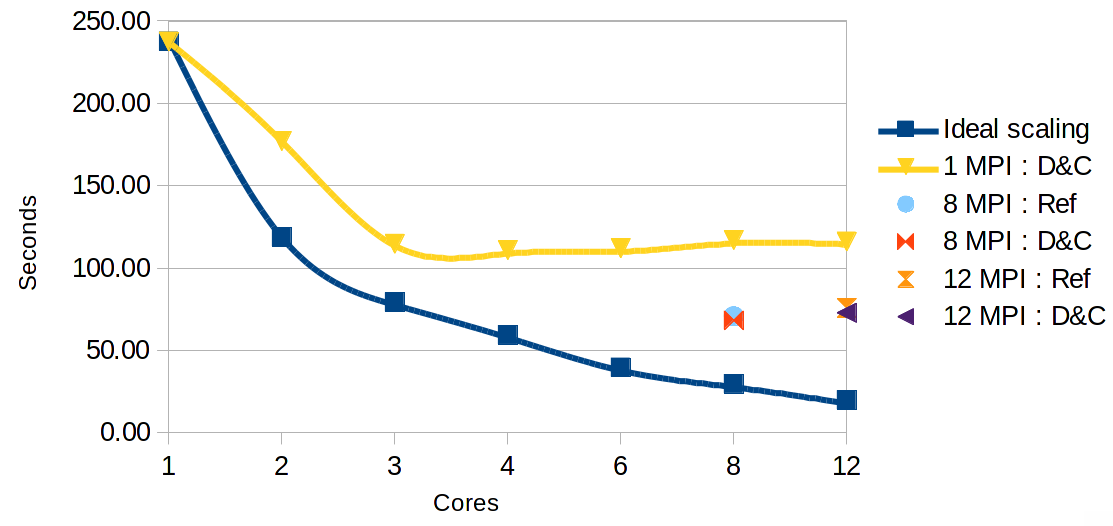
\includegraphics[scale=0.2]{Elasticity_solver_time.png}
 \caption{Elasticity solver execution time}
\end{figure}
As we can see in the 4 MPI curves and for the same reasons than in the Laplacian solver, the D\&C version is still a little bit faster than the original version.
We can expect even better results when the solver will be properly parallelized.
Further investigation are needed to evaluate why the pure MPI version does not scale perfectly in our experiments.

\section{Conclusion and Futur Work}
Assembly is only the 5 first percent of the DEFMESH application, but this is the starting point.
This step can represent much more time in other mesh deformation codes such has seismic simulation like SpecFem3D.
Hardware counters already show that vertex and elements reordering bring substantial improvements on data locality.
We also show a global improvement on RAM usage (?) etc...
The next step will be to work on the solver stage, using similar principles to enhance scalability and efficiency.
Extension will focus on D\&C friendly data structure definition, using D\&C on other part of the application such as the SpMV product or the iterative solver. 

\bibliographystyle{unsrt}
\bibliography{dc_bib}

\end{document}